\documentclass[
10pt, % Main document font size
a4paper, % Paper type, use 'letterpaper' for US Letter paper
oneside, % One page layout (no page indentation)
%twoside, % Two page layout (page indentation for binding and different headers)
headinclude,footinclude, % Extra spacing for the header and footer
BCOR5mm, % Binding correction
]{scrartcl}

%%%%%%%%%%%%%%%%%%%%%%%%%%%%%%%%%%%%%%%%%
% Arsclassica Article
% Structure Specification File
%
% This file has been downloaded from:
% http://www.LaTeXTemplates.com
%
% Original author:
% Lorenzo Pantieri (http://www.lorenzopantieri.net) with extensive modifications by:
% Vel (vel@latextemplates.com)
%
% License:
% CC BY-NC-SA 3.0 (http://creativecommons.org/licenses/by-nc-sa/3.0/)
%
%%%%%%%%%%%%%%%%%%%%%%%%%%%%%%%%%%%%%%%%%

%----------------------------------------------------------------------------------------
%	REQUIRED PACKAGES
%----------------------------------------------------------------------------------------

\usepackage[
nochapters, % Turn off chapters since this is an article        
beramono, % Use the Bera Mono font for monospaced text (\texttt)
eulermath,% Use the Euler font for mathematics
pdfspacing, % Makes use of pdftex’ letter spacing capabilities via the microtype package
dottedtoc % Dotted lines leading to the page numbers in the table of contents
]{classicthesis} % The layout is based on the Classic Thesis style

\usepackage{arsclassica} % Modifies the Classic Thesis package

\usepackage[T1]{fontenc} % Use 8-bit encoding that has 256 glyphs

\usepackage[utf8]{inputenc} % Required for including letters with accents

\usepackage{graphicx} % Required for including images
\graphicspath{{Figures/}} % Set the default folder for images

\usepackage{enumitem} % Required for manipulating the whitespace between and within lists

\usepackage{lipsum} % Used for inserting dummy 'Lorem ipsum' text into the template

\usepackage{subfig} % Required for creating figures with multiple parts (subfigures)

\usepackage{amsmath,amssymb,amsthm} % For including math equations, theorems, symbols, etc

\usepackage{varioref} % More descriptive referencing

%----------------------------------------------------------------------------------------
%	THEOREM STYLES
%---------------------------------------------------------------------------------------

\theoremstyle{definition} % Define theorem styles here based on the definition style (used for definitions and examples)
\newtheorem{definition}{Definition}

\theoremstyle{plain} % Define theorem styles here based on the plain style (used for theorems, lemmas, propositions)
\newtheorem{theorem}{Theorem}

\theoremstyle{remark} % Define theorem styles here based on the remark style (used for remarks and notes)

%----------------------------------------------------------------------------------------
%	HYPERLINKS
%---------------------------------------------------------------------------------------

\hypersetup{
%draft, % Uncomment to remove all links (useful for printing in black and white)
colorlinks=true, breaklinks=true, bookmarks=true,bookmarksnumbered,
urlcolor=webbrown, linkcolor=RoyalBlue, citecolor=webgreen, % Link colors
pdftitle={}, % PDF title
pdfauthor={\textcopyright}, % PDF Author
pdfsubject={}, % PDF Subject
pdfkeywords={}, % PDF Keywords
pdfcreator={pdfLaTeX}, % PDF Creator
pdfproducer={LaTeX with hyperref and ClassicThesis} % PDF producer
}
\usepackage{cite}
\usepackage{adjustbox}
\usepackage{booktabs}
\hyphenation{Fortran hy-phen-ation} 
\captionsetup{font=footnotesize}
\usepackage{booktabs}
\usepackage{enumitem}
\usepackage{tabularx, makecell}%
\renewcommand\theadfont{\normalsize\bfseries}
        \usepackage{etoolbox} %
        \AtBeginEnvironment{tabularx}{\setlist[enumerate, 1]{wide, leftmargin=*, itemsep=0pt, before=\vspace{-\dimexpr\baselineskip +2 \partopsep}, after=\vspace{-\baselineskip}}}

%----------------------------------------------------------------------------------------
%	TITLE AND AUTHOR(S)
%----------------------------------------------------------------------------------------
\title{\normalfont\spacedallcaps{}} % The article title

%\author{\spacedlowsmallcaps{Fatemeh Hadi Nezhad\textsuperscript{1}}}

%\date{2019} % An optional date to appear under the author(s)

%----------------------------------------------------------------------------------------

\begin{document}

%----------------------------------------------------------------------------------------
%	HEADERS
%----------------------------------------------------------------------------------------

\renewcommand{\sectionmark}[1]{\markright{\spacedlowsmallcaps{#1}}} % The header for all pages 
\lehead{\mbox{\llap{\small\thepage\kern1em\color{halfgray} \vline}\color{halfgray}\hspace{0.5em}\rightmark\hfil}} % The header style

\pagestyle{scrheadings} % Enable the headers specified in this block

%----------------------------------------------------------------------------------------
%	TABLE OF CONTENTS & LISTS OF FIGURES AND TABLES
%----------------------------------------------------------------------------------------

%\maketitle % Print the title/author/date block

\setcounter{tocdepth}{3} % Set the depth of the table of contents to show sections and subsections only

\tableofcontents % Print the table of contents

%----------------------------------------------------------------------------------------
%	AUTHOR AFFILIATIONS
%----------------------------------------------------------------------------------------

%\let\thefootnote\relax\footnotetext{* \textit{Department of Quantitative System Biology, University of California, Merced, United States}}

%----------------------------------------------------------------------------------------

\newpage 

%----------------------------------------------------------------------------------------
%	Preparing Data
%----------------------------------------------------------------------------------------

\section{Preparing Data}
%------------------------------------------------
\textbf{TryTryp genome data}. From tritrypdb website, we downloaded the version 41 of 46 TryTryp genomes released on 2018-12-05. Genomes are compared based on number of sequence fragments relative to their length as shown in figure ~\vref{fig:gallery}. 
All the results, scripts for TryTryp version 41 can be found \href{https://github.com/fhadinezhadUC/Leishmania_2019}{here}. 

\begin{figure}[tb]
\centering 
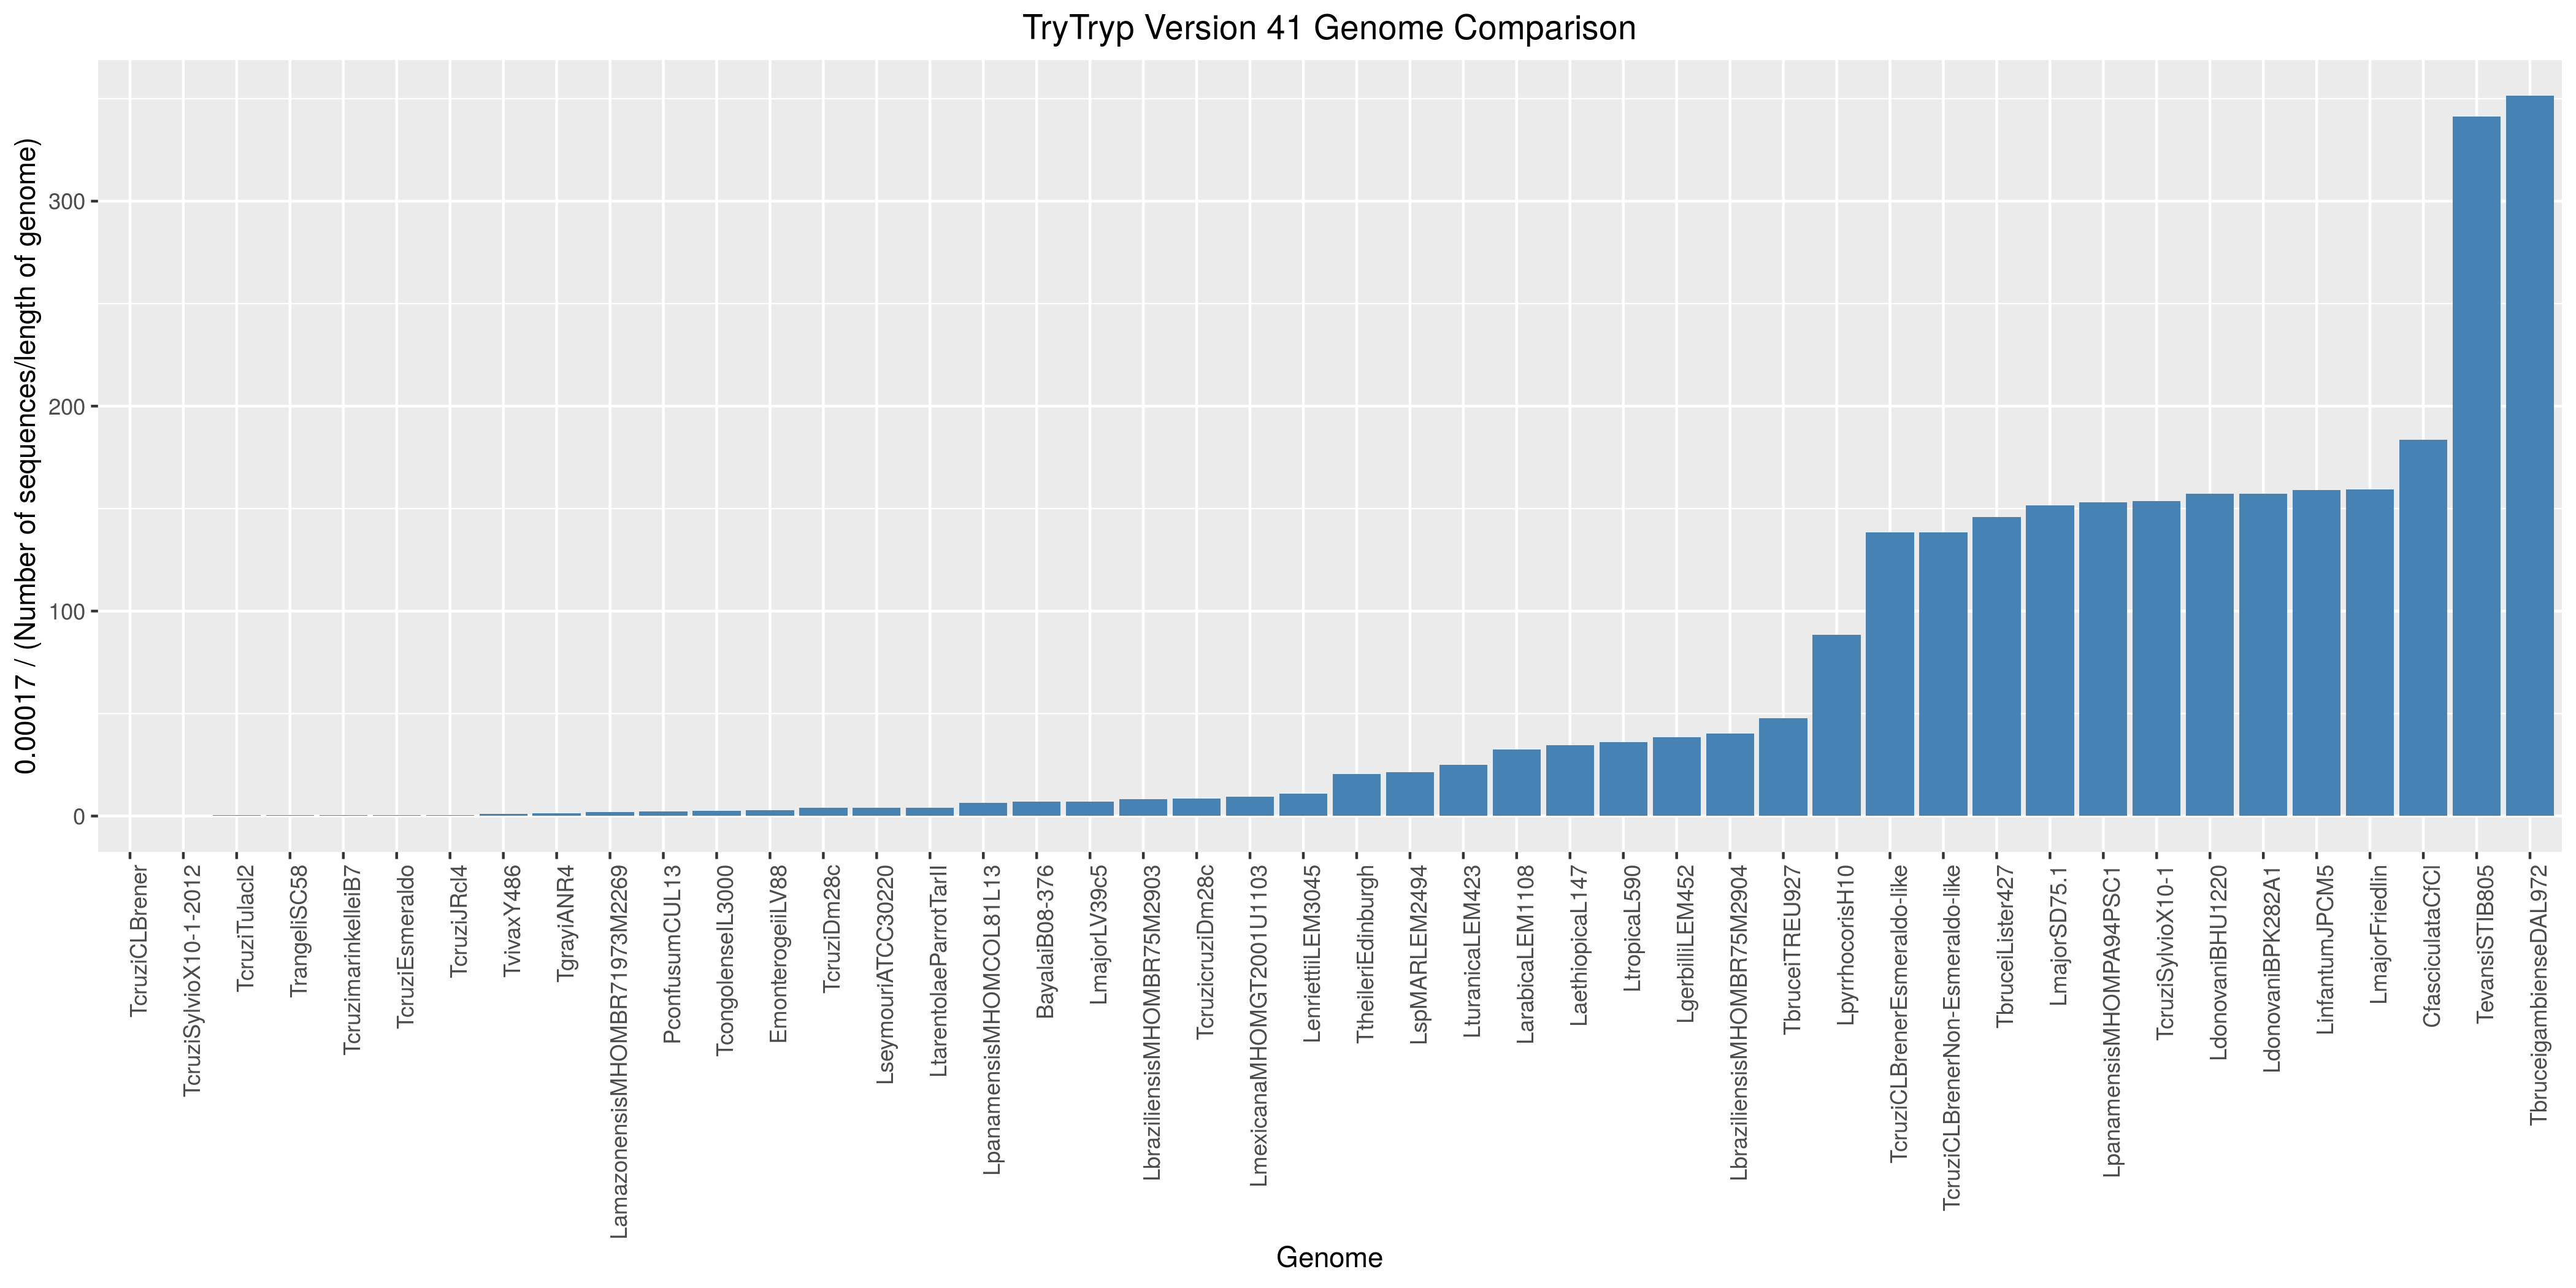
\includegraphics[width=0.8\columnwidth]{GenomeComparisonV41.png} 
\caption[Genome Comparison]{Comparing genomes based on formula ${(\frac{f(x)}{\max(f(x))})}^{-1}$. f(x) = Number of sequences in genome devided by the length of genome. The length of the bars shows how good the genomes are sequenced.} % The text in the square bracket is the caption for the list of figures while the text in the curly brackets is the figure caption
\label{fig:gallery} 
\end{figure}

\subsection{\textbf{tRNA gene annotation}}
\subsubsection{tRNA gene prediction}
In order to annotate tRNA genes for the sequenced TryTryp genomes, we used two computational methods for tRNA prediction, tRNAscan-SE and Aragorn. We integrated the result of both genefinders by keeping the union of tRNA gene predictions generated by tRNAscan-SE v2.0 using defult options (Lowe and Eddy 1997) and Aragorn v1.2.38 using options -i116 -t -br -seq -w -e -l -d (Laslett and Canback 2004). Genes with overlapped coordinate were considered as one gene. However, the identity and exact coordinate of both genefinders we saved seperately to be analysed later. 

%----------------------------------------------------------------------------------------
%	Initiator tRNA prediction
%----------------------------------------------------------------------------------------

\subsubsection{Initiator tRNA prediction}
We predicted the initiator tRNAs for the genes with anticodon 'CAT' from intersection of both tRNAscan (TSE) and Aragorn (ARA) Based on Conserved positions of initiators in Eukarya from the study by CHRISTIAN MARCK and HENRI GROSJEAN. Based on this study we have the fallowing citeria for initiators:
\begin{enumerate}[noitemsep] % [noitemsep] removes whitespace between the items for a compact look
\item In all eukaryotic tDNA-iMet, positions 11–24 are occupied by C-G, However, eukaryotic elongators
also prefer C-G at these positions.

\item Initiator tDNAs from Eukarya use A54 and A60. Some eukaryotic elongators also use either A54 or
A60 but none (with only one exception) uses both

\item Initiator tDNA-iMet (CAT) from all domains display the GGG sequence (Mandal et al+, 1996) or,
very seldom, the AGG sequence at positions 29 to 31, pairing with the complementary CCC or
CCT sequences at positions 39 to 41

\item Another domain-specific feature in all eukaryotic initiators is the systematic nonoccupancy of all
optional positions of the D-loop (17, 17a, 20a, and 20b) whereas in elongators, only position 17a is always unoccupied.

\item At position 20, A is strictly conserved in all eukaryotic initiators
\end{enumerate} 
To investigate all these features we clustered CAT tRNA genes using Levenshtein (edit) distance between gene sequences and Ward.D2 method to measure the dissimilarity between each two clusters. We ended up with three clusters. Table \ref{table:1} investigates each of these features in each column. from this table we see that only tRNA genes in cluster 1 have almost all the conserved features for eukaryotic initiators. So, we marked these genes as initiators represented with letter X in our gene file.


\begin{table}[hbt]
\caption{Table of CAT clusters to show how many tRNA genes in each cluster satisfy each feature}
\begin{adjustbox}{width=\columnwidth,center}
%\caption{Table of Grades}
%\centering
\begin{tabular}{|l|lllllllll|}
\hline
Clusters & \# tRNAs & 11–24(C-G) & 54-60(A-A)(T-T) & 1-72(A-T) & 29-31(GGG) & 39-41(CCC/CCT) & \#  posisInDloop & 20A & distanceRange \\
\hline
Cluster1 & 76 & 76 & 76 & 76 & 76 & 76 & 7 & 75 & 0-6\\
Cluster2 & 95 & 95 & 2 & 0 & 95 & 95 & 8 & 0 & 0-8\\
Cluster3 & 2 & 2 & 2 & 0 & 0 & 0 & 8/9 & 0 & 0-22\\
\hline
\end{tabular}
\label{table:1}
\end{adjustbox}
\end{table}



%----------------------------------------------------------------------------------------
%	tRNA Genes Integration
%----------------------------------------------------------------------------------------

\subsection{\textbf{Summary of predicted TryTryp tRNA genes}}

To investigate and compare tRNA genes predicted by two gene finders TSE and ARA, we made four sets of genes. Set one, TSE and ARA intersection, Set two, TSE and ARA union, Set three, genes found by ARA and Set four, genes found by TSE . for intersection set, we dismissed genes which had different identity by ARA and TSE. for union set, we picked TSE identity over ARA. Table  ~\ref{table:2} shows a summary of these four sets. Further, to compare the coordinates of genes annotated by ARA and TSE we made a heatmap shown in figure ~\ref{fig:heatmap}. We see from this figure that the coordinates of same genes annotated by ARA and TSE do not always match. We Analysed the reason for each set of displacementin this figure as fallow:

\begin{enumerate}[noitemsep]

\item Genes with 0 displacement in both ends: These genes have same identity for both TSE and ARA except for 33 genes with Anticodon loop of more than 8bp. Also, both ARA and TSE reported genes up to base 73. 
\item Genes with 0 displacement at 5 prime end and 1 displacement at 3 prime end: Identity of these genes matches between ARA and TSE. They all have anticodon loop of length 7. The reason for the displacement in 3 prime end is that ARA reports up to position 74, however, TSE reports only up to position 73.  
\item Genes with one base displacement at both ends: In this case ARA reports one extra base at both ends which is because these two bases pair together and in most cases this makes the Amino Acid arm one base longer than what TSE reports. Although in a few cases, the AminoAcid arm will stay 7bp, but we see insertions in this arm.  
\item Genes with two base displacement at 3 prime end and one at 5 prime end: In this case ARA is reporting 2 extra bases at one end and 1 for the other end which usually leads to a longer AminoAcid arm. Also, the extra 2 bases reported by ARA at 3 prime end are mostly 'ac'.  
\item Genes with two base displacement at 3 prime end and 0 displacement at 5 prime end: In this case TSE reports up to position 73 as always, but ARA is reporting genes up to position 75. the last three bases of ARA are mainly 'acc'
\item Genes with three base displacement at 3 prime end and 0 displacement at 5 prime end. In this case ARA is reporting 3 extra bases at 3 prime end and these three bases are '?cc'.


\end{enumerate} 

%----------------------------------------------------------------------------------------
%	???? Analyse why we have the differences ....
%----------------------------------------------------------------------------------------

We expect our genefinders to annotate tRNA genes of all 22 functional classes for each genome. To investigate this we visualized the number of genes annotated for each genome in Figure ~\ref{fig:counts} and tRNA functional classes annotated by both TSE and ARA for each genome in Figure ~\ref{fig:types}.

\begin{table}[hbt]
\caption{summary of the predicted genes by TSE and ARA. We marked pseudo genes as \$, initiators as X, stop as \#, sup as "?", sec as Z and pyl as O}
\begin{adjustbox}{width=\columnwidth,center}
%\caption{Table of Grades}
%\centering
% make it as two table
\begin{tabular}{|l|lllllllllllllllllllllllllllllllllll|}
\hline
GeneSet & \# tRNA & \# nucleotides & N/T & gene length & \%G & \%C & \%T & \%A & \%intron & A & C & D & E & F & G & H & I & K & L & M & N & P & Q & R & S & T & V & W & Y & X & Z & \$ & ? & \# & O\\
TSE2 & 3631 & 270355 & 74.46 & 50-164 & 31.99 & 26.11 & 23.22 & 18.68 &  2.616 & 214 & 64 & 105 & 163 & 110 & 234 &  80 & 179 & 190 & 338 & 108 & 126 & 201 & 162 & 350 & 238 & 219 & 241 & 52 &  94 & 76 & 78 & 28 & 3 & 0 & 0\\
ARA & 4347 & 372539 & 85.70 & 70-215 & 32.64 & 26.92 & 22.87 & 17.57 & 14.677 & 257 & 86 & 124 & 193 & 125 & 339 & 129 & 213 & 194 & 393 & 101 & 153 & 228 & 175 & 420 & 362 & 248 & 282 & 60 &  90 & 76 & 82 &  0 & 0 & 2 & 4\\
UNION & 4381 & 377734 & 86.22 & 50-215 & 32.81 & 26.66 & 22.87 & 17.65 & 15.339 & 259 & 86 & 119 & 194 & 130 & 344 & 129 & 220 & 197 & 380 & 112 & 143 & 229 & 175 & 421 & 369 & 249 & 282 & 57 & 106 & 76 & 82 & 28 & 3 & 2 & 2\\
INTERSECTION & 3562 & 265160 & 74.44 & 68-89 & 32.01 & 26.13 & 23.22 & 18.64 &  2.330 & 212 & 64 & 105 & 162 & 105 & 229 &  80 & 172 & 187 & 338 &  97 & 125 & 200 & 162 & 349 & 230 & 218 & 241 & 52 &  78 & 76 & 78 &  6 & 0 & 0 & 0\\
\hline
\end{tabular}
\label{table:2}
\end{adjustbox}
\end{table}


\begin{figure}[tb]
\centering 
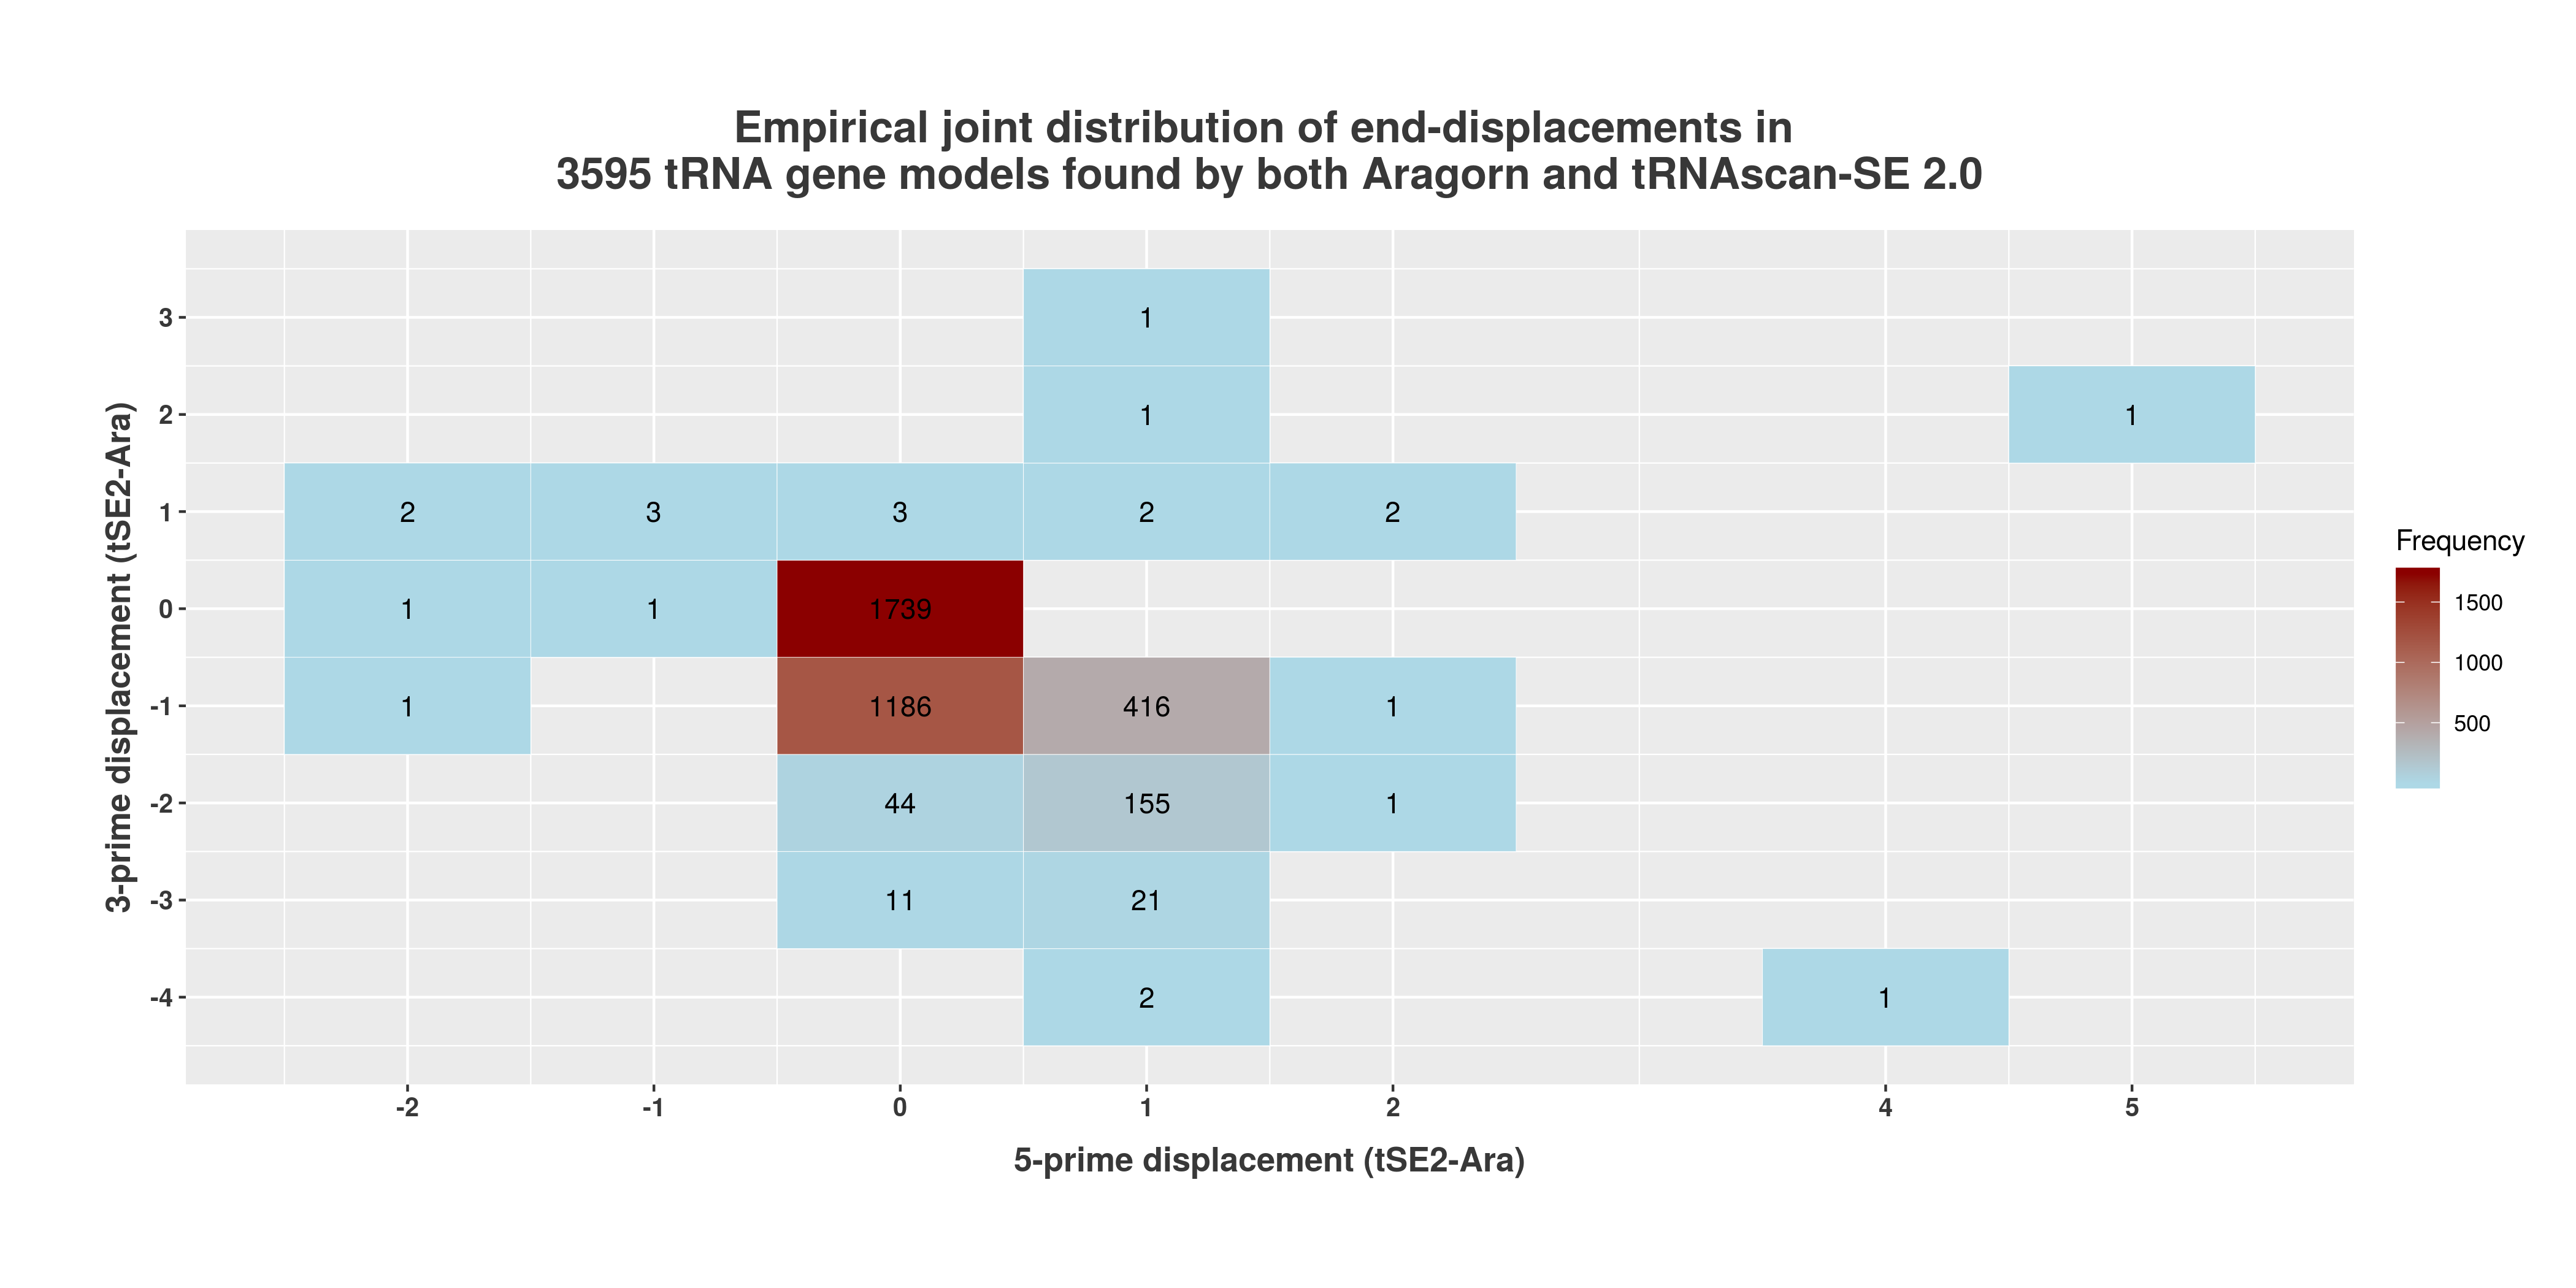
\includegraphics[width=0.8\columnwidth]{EndDisplacement.png} 
\caption[Genome Comparison]{Empirical joint distribution of end-displacements in ? tRNA gene models found by both Aragorn and tRNAscan-SE 2.0.} % The text in the square bracket is the caption for the list of figures while the text in the curly brackets is the figure caption
\label{fig:heatmap} 
\end{figure}
 
\begin{figure}[tb]
\centering 
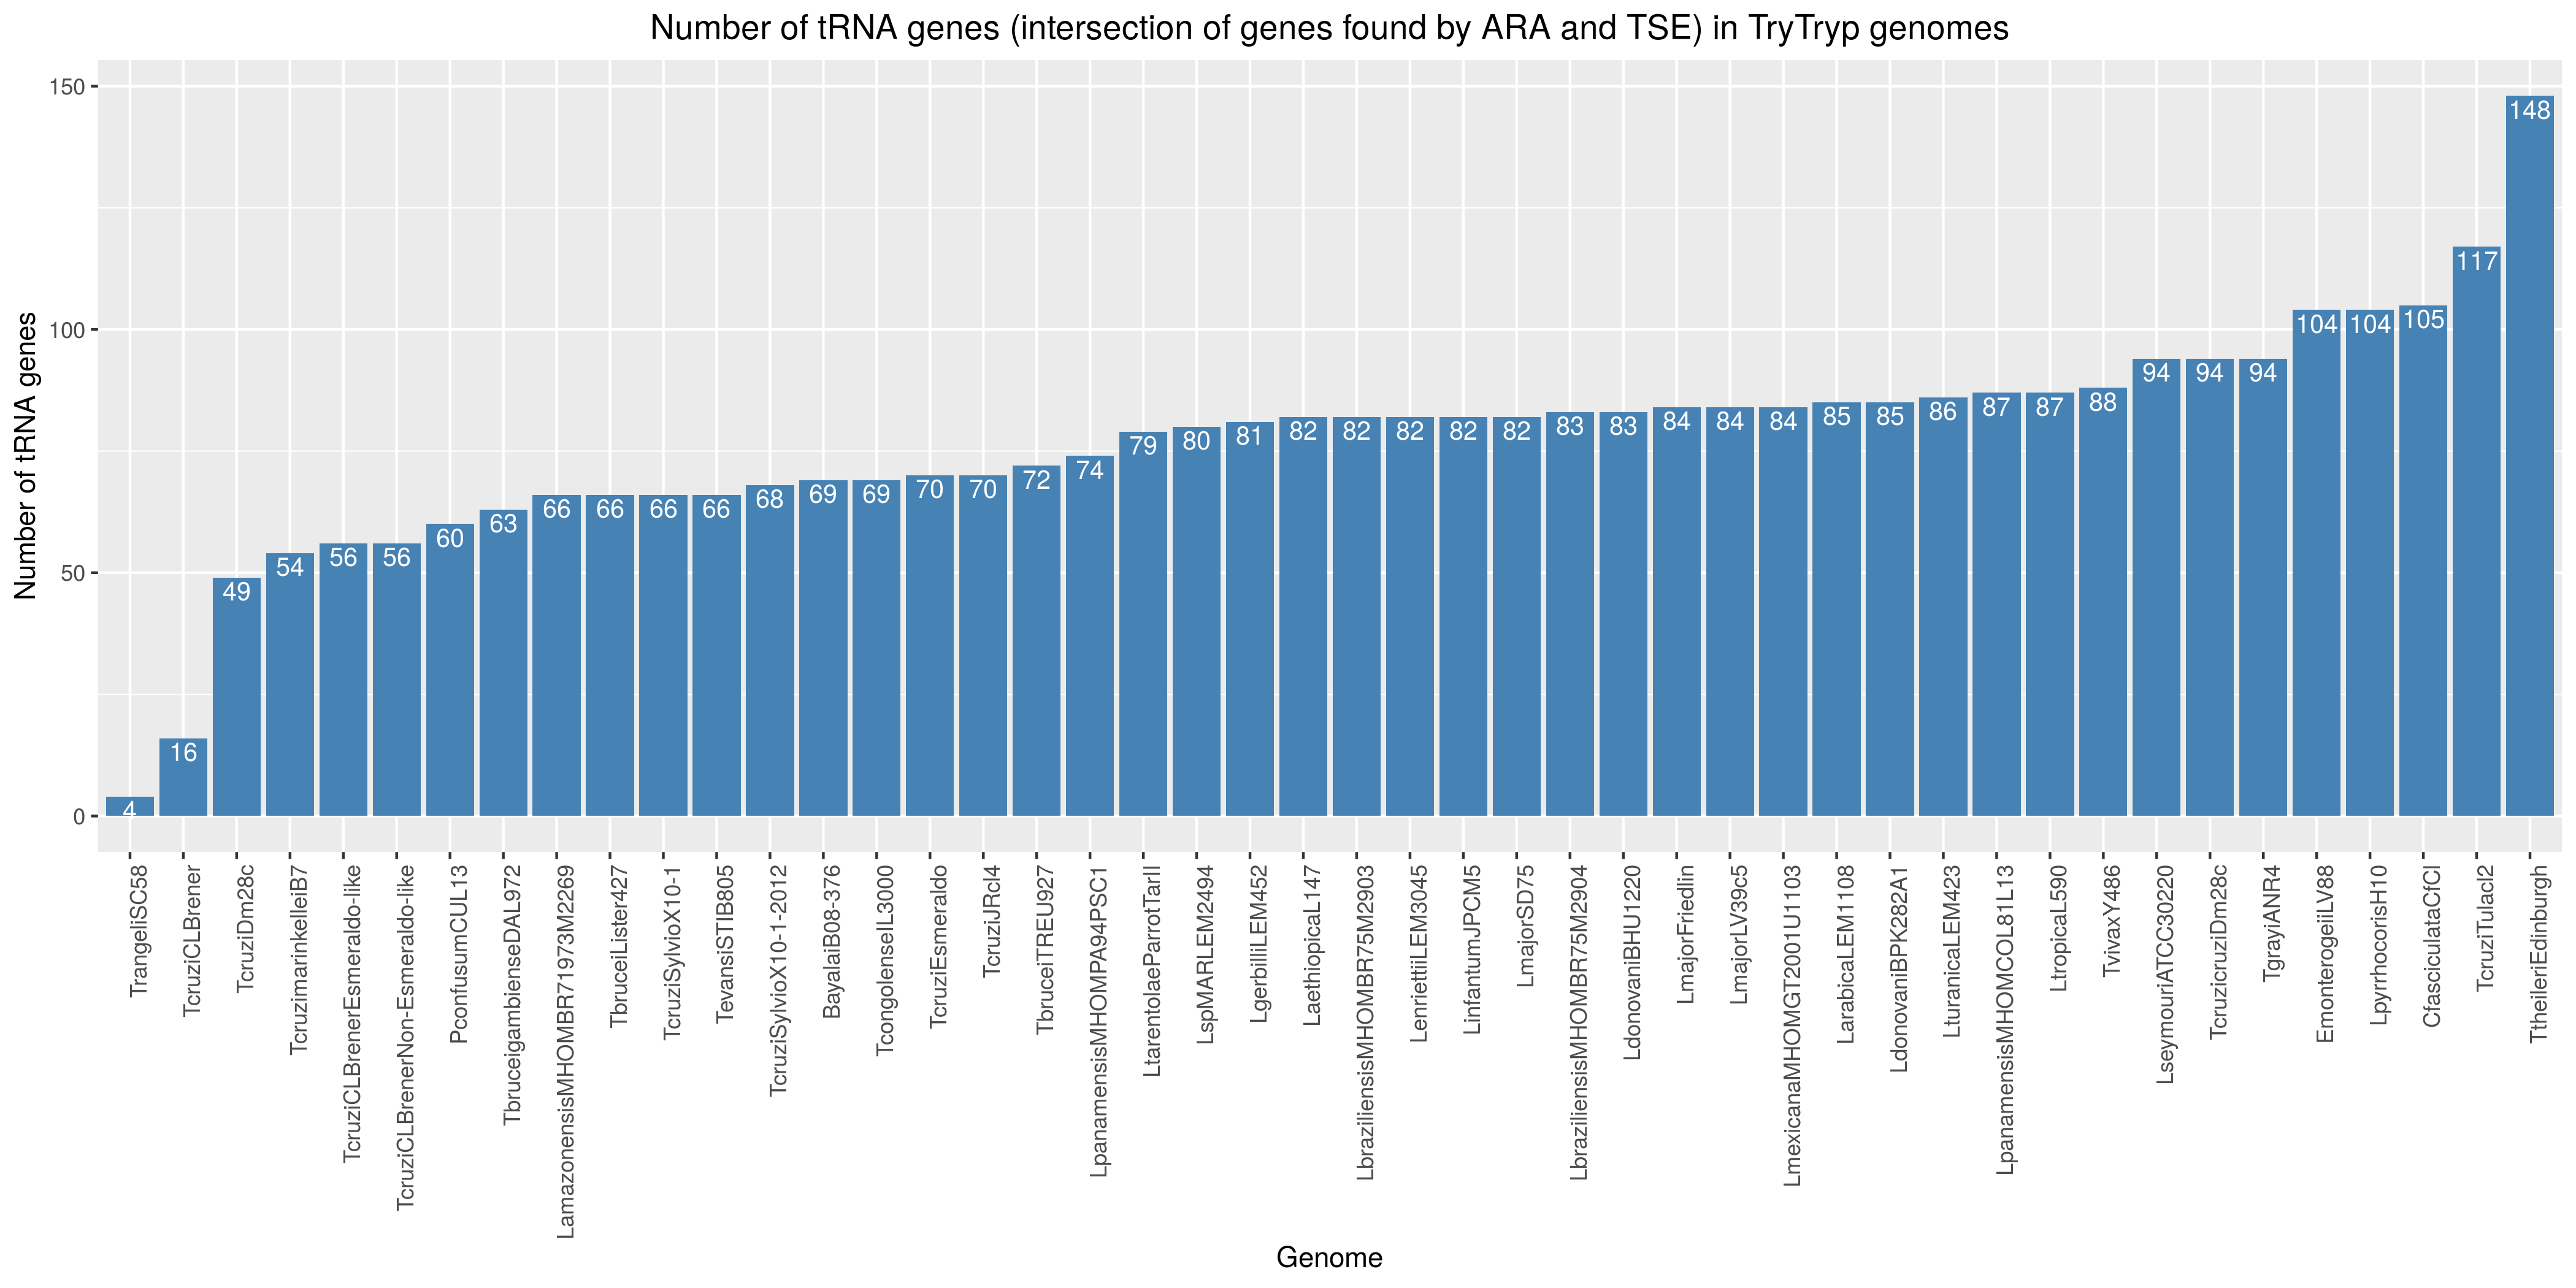
\includegraphics[width=0.8\columnwidth]{intersecttRNAcounts.png} 
\caption[Number of Genes annotated]{Number of genes annotated by both TSE and ARA for each TryTryp genome.} % The text in the square bracket is the caption for the list of figures while the text in the curly brackets is the figure caption
\label{fig:counts} 
\end{figure}

\begin{figure}[tb]
\centering 
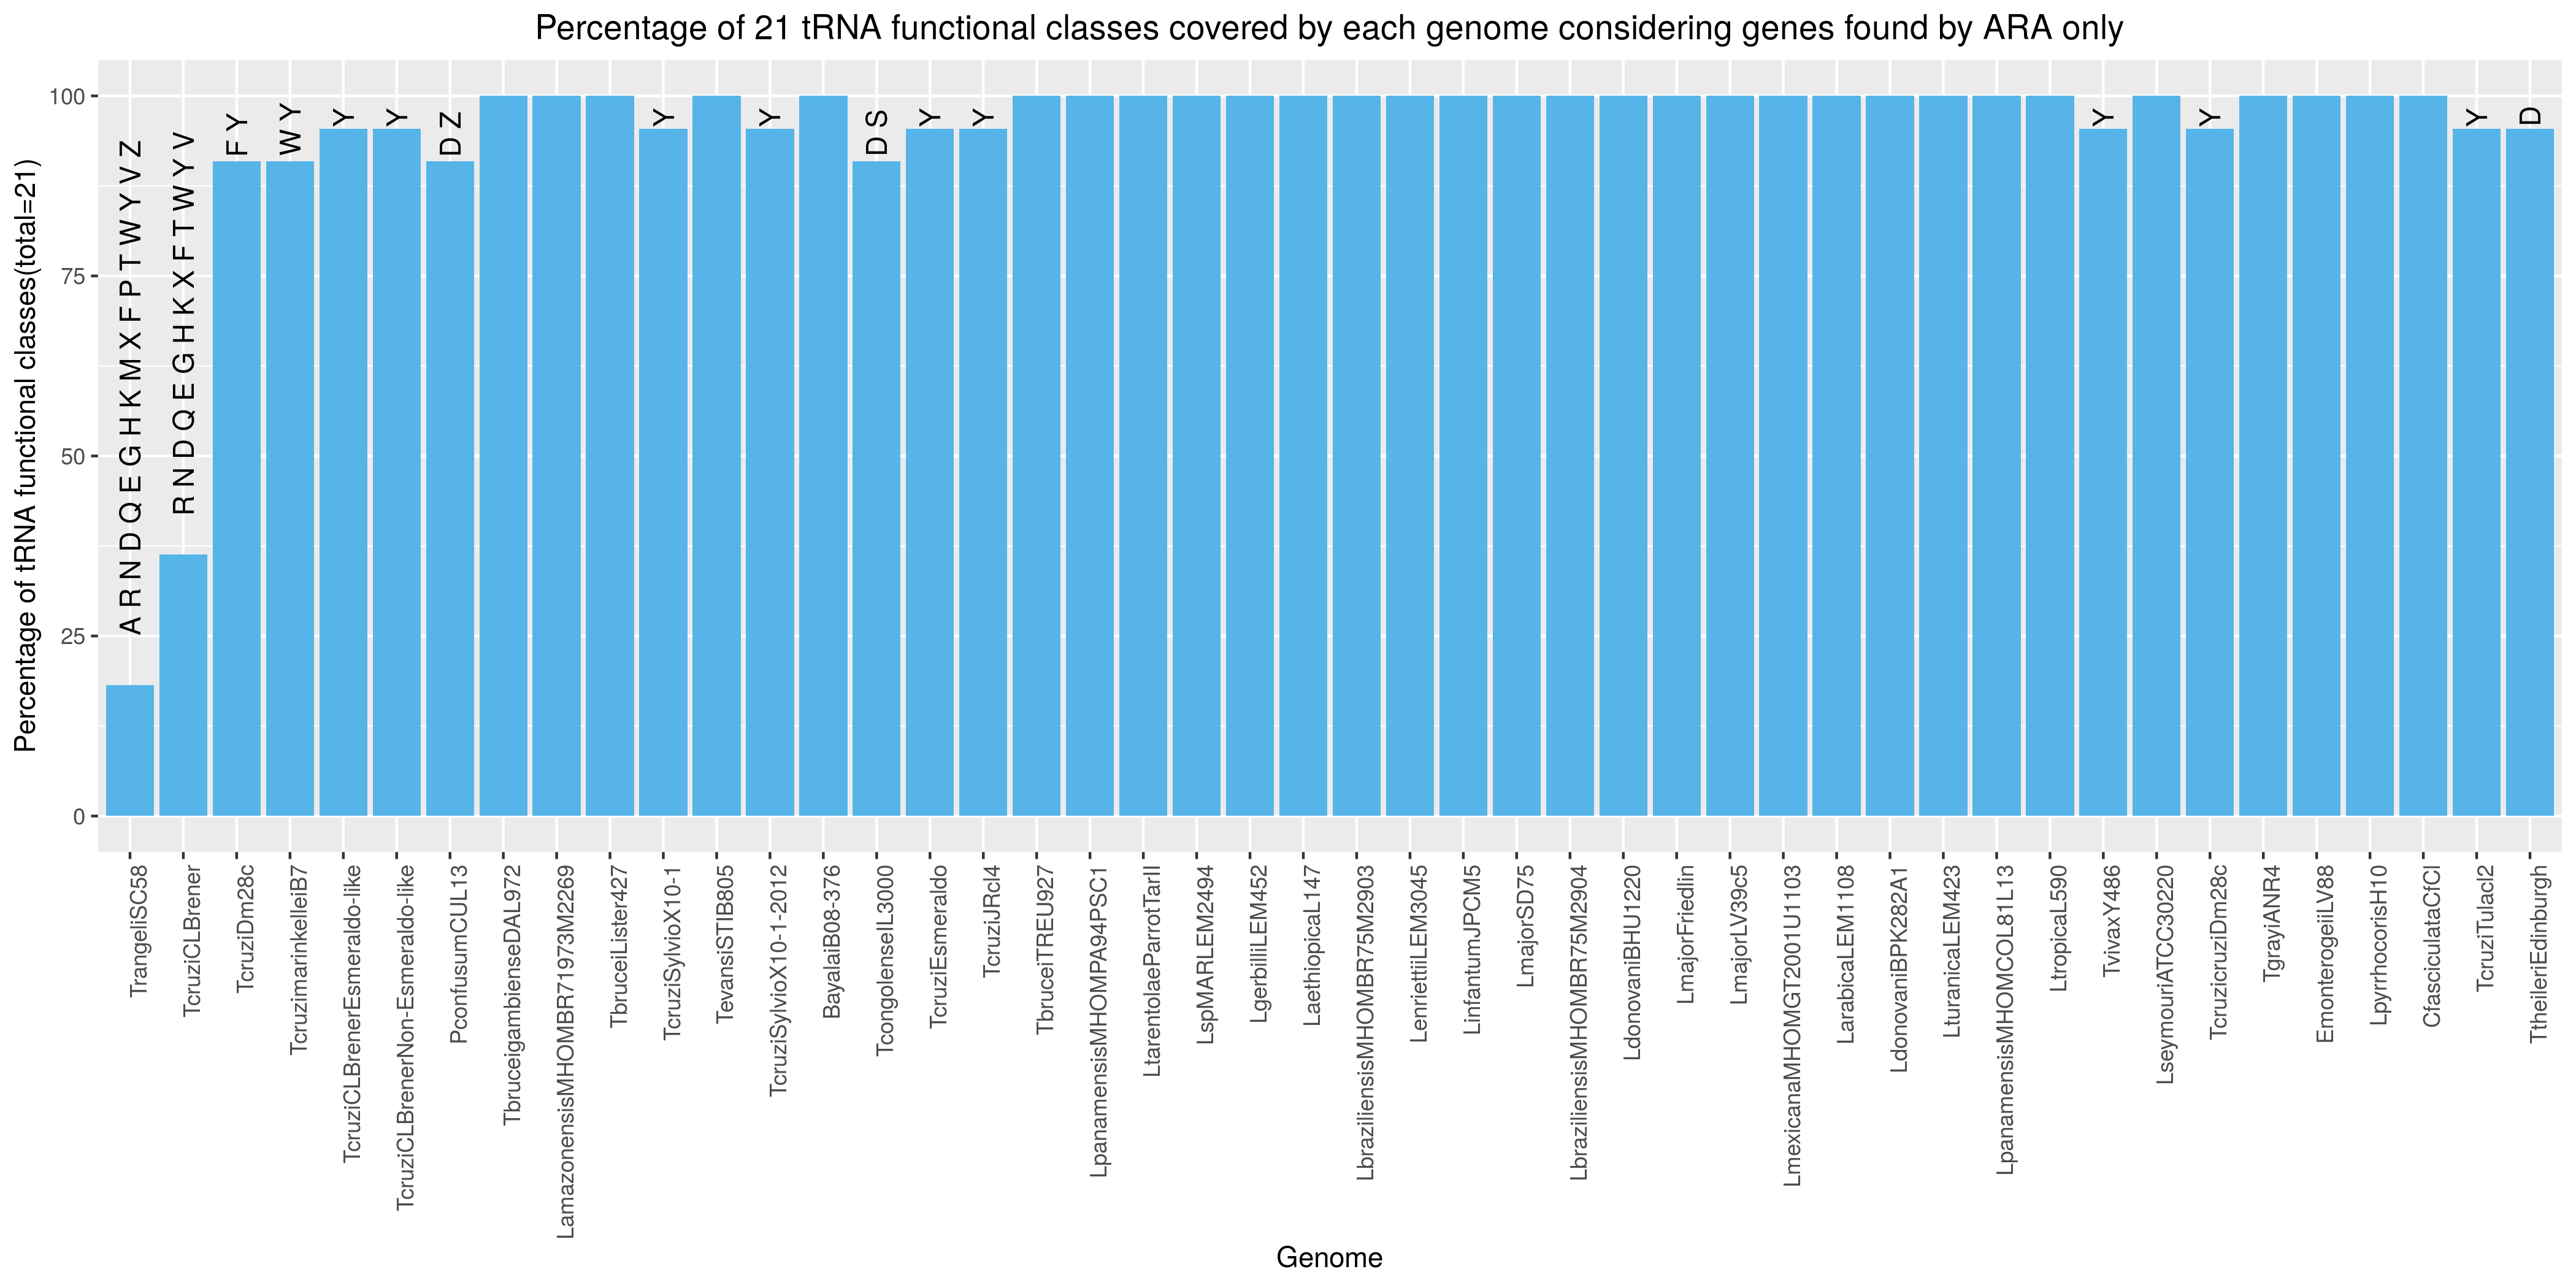
\includegraphics[width=0.8\columnwidth]{ara_funcPerc.png} 
\caption[Genome Comparison]{Percentage of 22 tRNA types annotated by both TSE and ARA for each TryTryp genomes. The label on top of each bar shows which tRNA classes are not annotated for the genome.} % The text in the square bracket is the caption for the list of figures while the text in the curly brackets is the figure caption
\label{fig:types} 
\end{figure}

from figure ~\ref{fig:counts} we see that few of the 22 tRNA classes are not annotaded for all the genomes. To improve the annotation we included 33 genes annotated by both gene finders, with mismatched identities. you can see a summary of these genes in table \ref{table:3}. 
To determind the identity of these genes we built a structural alignment of all the TryTryp tRNA genes from our intersection set and 33 genes (We picked TSE reported sequences over ARA for alignment, because TSE reports genes up to position 73, however ARA can report a few bases after 73 as we see in figure \ref{fig:heatmap}. We used removed introns and other nucleotides in non-conserved positions, and variable arms prior to the alignment. We used covea v2.4.2 (Sean Eddy 1994) for the structural alignment and edited the alignment by removing sites with more than 99\% gap, genes with more than 8 gaps in their aligned sequence, and genes with letter N in their sequence.). Later, using only the intersection aligned genes we made a profile covariance model for 22 functional classes. We calculated the score of 33 genes for each of these 22 models. For each gene, we compared the score of two models made for the indentities reported by TSE and ARA and picked the one with higher score. you can see the result in this \href{https://github.com/fhadinezhadUC/Leishmania_2019/blob/master/Results/Integrated_Genes/UndetClassScore.txt} {file}. We were able to include 32 of these genes to our intersection set which improved the annotation of genomes as you can see in figure \ref{fig:typesimproved}


\begin{table}[hbt]
\caption{33 genes annotated by both TSE and ARA with mismatched identity}
\begin{adjustbox}{center}
%\caption{Table of Grades}
%\centering
\scalebox{0.7}{
\begin{tabular}{|l|llllllll|}
\hline
ARA|TSE & D|I & L|? & L|E & L|M & N|Y & O|M & S|R & W|G\\
\hline
Number of genes &5  & 3  & 1 &  9 & 11 &  2 &  1 &  3 \\
\hline
\end{tabular}
}
\label{table:3}
\end{adjustbox}
\end{table}


\begin{figure}[tb]
\centering 
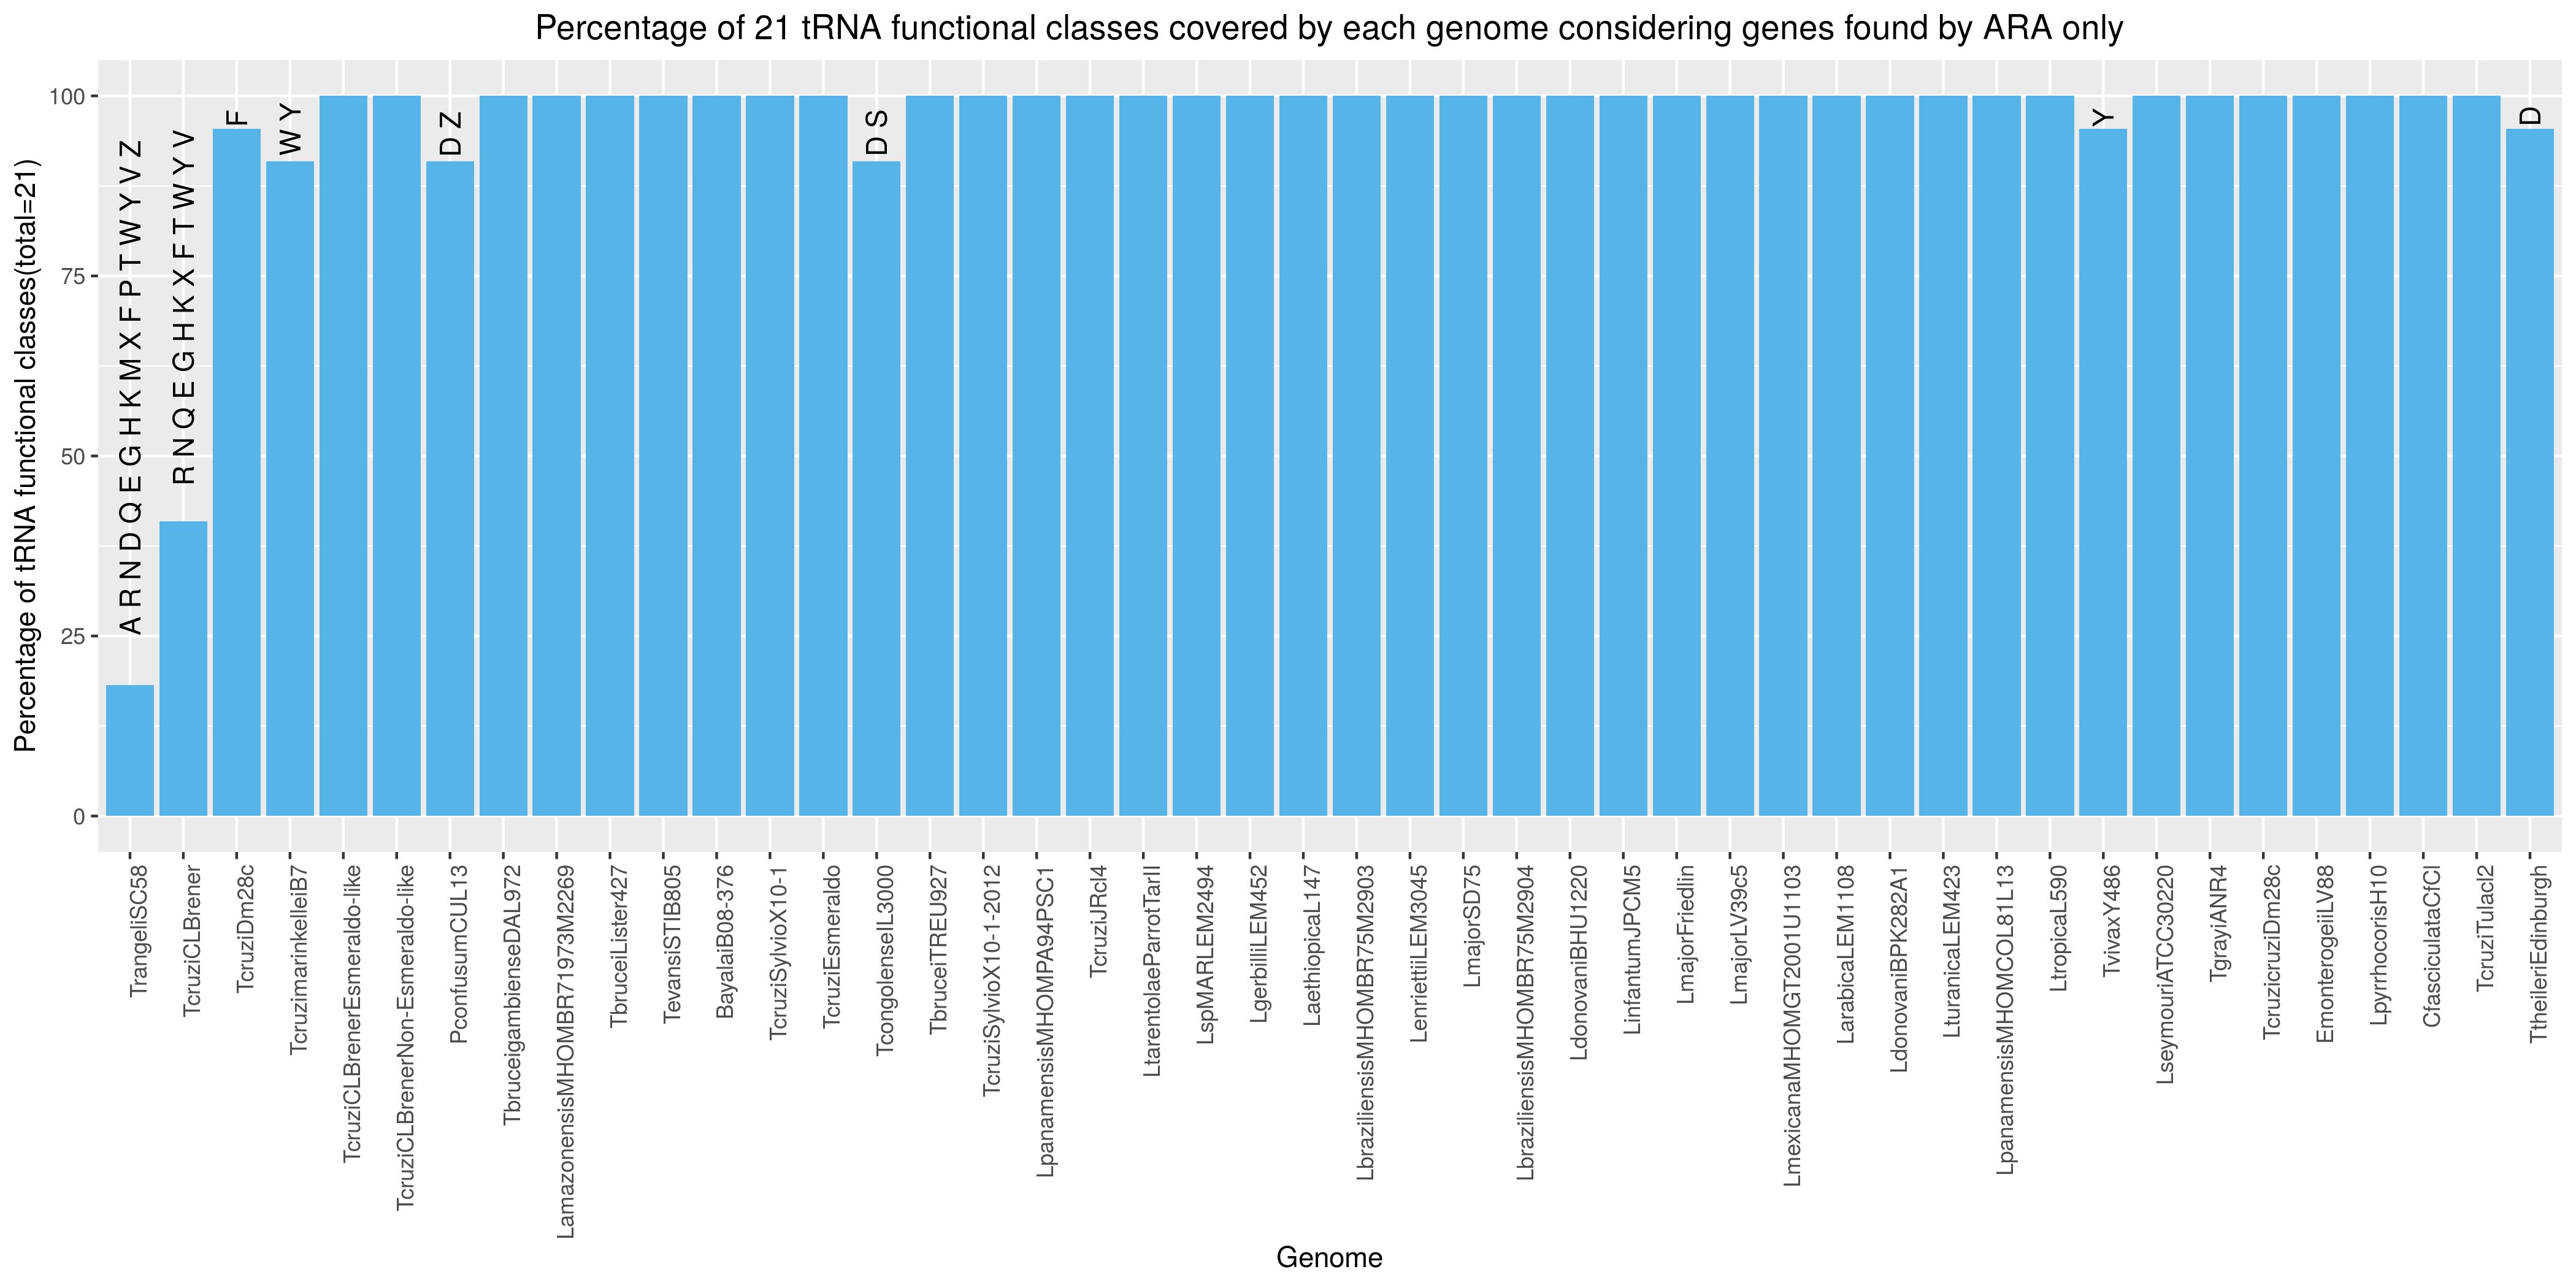
\includegraphics[width=0.8\columnwidth]{ara_funcPerc2.png} 
\caption[Genome Comparison]{Percentage of 22 tRNA types annotated by both TSE and ARA for each TryTryp genomes after including 32 genes to intersection set. The label on top of each bar shows which tRNA classes are not annotated for the genome.} % The text in the square bracket is the caption for the list of figures while the text in the curly brackets is the figure caption
\label{fig:typesimproved} 
\end{figure}

\section{TryTryp Classification}


We visualized differences in tRNA identity determinants between TryTryp and Human, and across TryTryp genomes, using four different Logos: 
\begin{enumerate}[noitemsep]

\item[1] Function Logos to estimate the potential identity determinants for each genome 
\item[2] Information Difference logos (ID logos), to show the evolutionary gain or loss of functional information between Human and TryTryp genomes 
\item[3] KullbackeLeibler divergence Difference logos (KLD logos) to show changes in the functional associations of features between Human and TryTryp genomes
\item[4] Using Three Logos mentioned above, we made bubble plots to show gains and shifts in functions of tRNAs in Trypanosomea contrasted against human tRNAs.

\end{enumerate}

Using phylogenetic trees of Trypanosoma from these works \cite{Souza:2018dg,Hughes:2003,Pothirat:2014,Kelly:2017}, we grouped TryTryp genomes as table \ref{table:4}. figure \ref{fig:countsclustered} shows a summery of the number of tRNA genes for each cluster and figure \ref{fig:funcclustered} shows the tRNA functional classes not annotated for clusters of genome. we excluded genome PconfusumCUL13 from the study, until we find a well sequenced version of this genome for which we can annotate all 22 functional classes of tRNAs. The Logo data for TryTryp genomes and Human can be found \href{https://github.com/fhadinezhadUC/Leishmania_2019/tree/master/Results/tsfmInput-output/output/Logos}{here}. you can find the bubble plots for each cluster \href{https://github.com/fhadinezhadUC/Leishmania_2019/tree/master/Results/tsfmInput-output/output/BubblePlots}{here}. we have 11 pages and each page has 21 models for all tRNA classes in a cluster. 
\begin{table}[hbt] 
\caption{Classification of TryTryp genomes. genomes not mentioned here are clustered as one genome.}
\begin{adjustbox}{width=\columnwidth,center}
\begin{tabular}{|c|c|c|c|c|c|c|c|}
        \toprule LenriettiComplex & AfricanTrypanosome & AmericanTrypanosome & Leishmania1 & Leishmania2 &LDonovaniComplex & LMexicanaComplex & Lvianna \\\midrule
        \parbox{.45\textwidth} {\begin{enumerate}
            \item LspMARLEM2494
            \item LenriettiiLEM3045
        \end{enumerate}} & \parbox{.45\textwidth}{\begin{enumerate}
            \item TbruceigambienseDAL972
            \item TbruceiLister427
            \item TbruceiTREU927
            \item TevansiSTIB805
            \item TcongolenseIL3000
            \item TvivaxY486
        \end{enumerate}} & \parbox{.45\textwidth}{\begin{enumerate}
            \item TgrayiANR4
            \item TrangeliSC58
            \item TcruziCLBrener
            \item TcruziCLBrenerEsmeraldo-like
            \item TcruziCLBrenerNon-Esmeraldo-like
            \item TcruzicruziDm28c
            \item TcruziDm28c
            \item TcruziEsmeraldo
            \item TcruziJRcl4
            \item TcruzimarinkelleiB7
            \item TcruziSylvioX10-1
            \item TcruziSylvioX10-1-2012
            \item TcruziTulacl2
            \item TtheileriEdinburgh
        \end{enumerate}} & \parbox{.45\textwidth}{\begin{enumerate}
            \item CfasciculataCfCl
            \item LseymouriATCC30220
            \item LpyrrhocorisH10
        \end{enumerate}}& \parbox{.45\textwidth}{\begin{enumerate}
            \item LmajorFriedlin
            \item LmajorLV39c5
            \item LmajorSD75
            \item LturanicaLEM423
            \item LarabicaLEM1108
            \item LtropicaL590
            \item LaethiopicaL147
            \item LgerbilliLEM452
        \end{enumerate}}& \parbox{.45\textwidth}{\begin{enumerate}
            \item LdonovaniBHU1220
            \item LdonovaniBPK282A1
            \item LinfantumJPCM5
        \end{enumerate}}& \parbox{.45\textwidth}{\begin{enumerate}
            \item Lamazonensis\\
                  MHOMBR71973M2269
            \item Lmexicana\\MHOMGT2001U1103
        \end{enumerate}}& \parbox{.45\textwidth}{\begin{enumerate}
            \item Lbraziliensis\\MHOMBR75M2904
            \item Lbraziliensis\\MHOMBR75M2903
            \item Lpanamensis\\MHOMPA94PSC1
            \item Lpanamensis\\MHOMCOL81L13
        \end{enumerate}}\\
        \bottomrule
\end{tabular}
\label{table:4}
\end{adjustbox}
\end{table}

\begin{figure}[tb]
\centering 
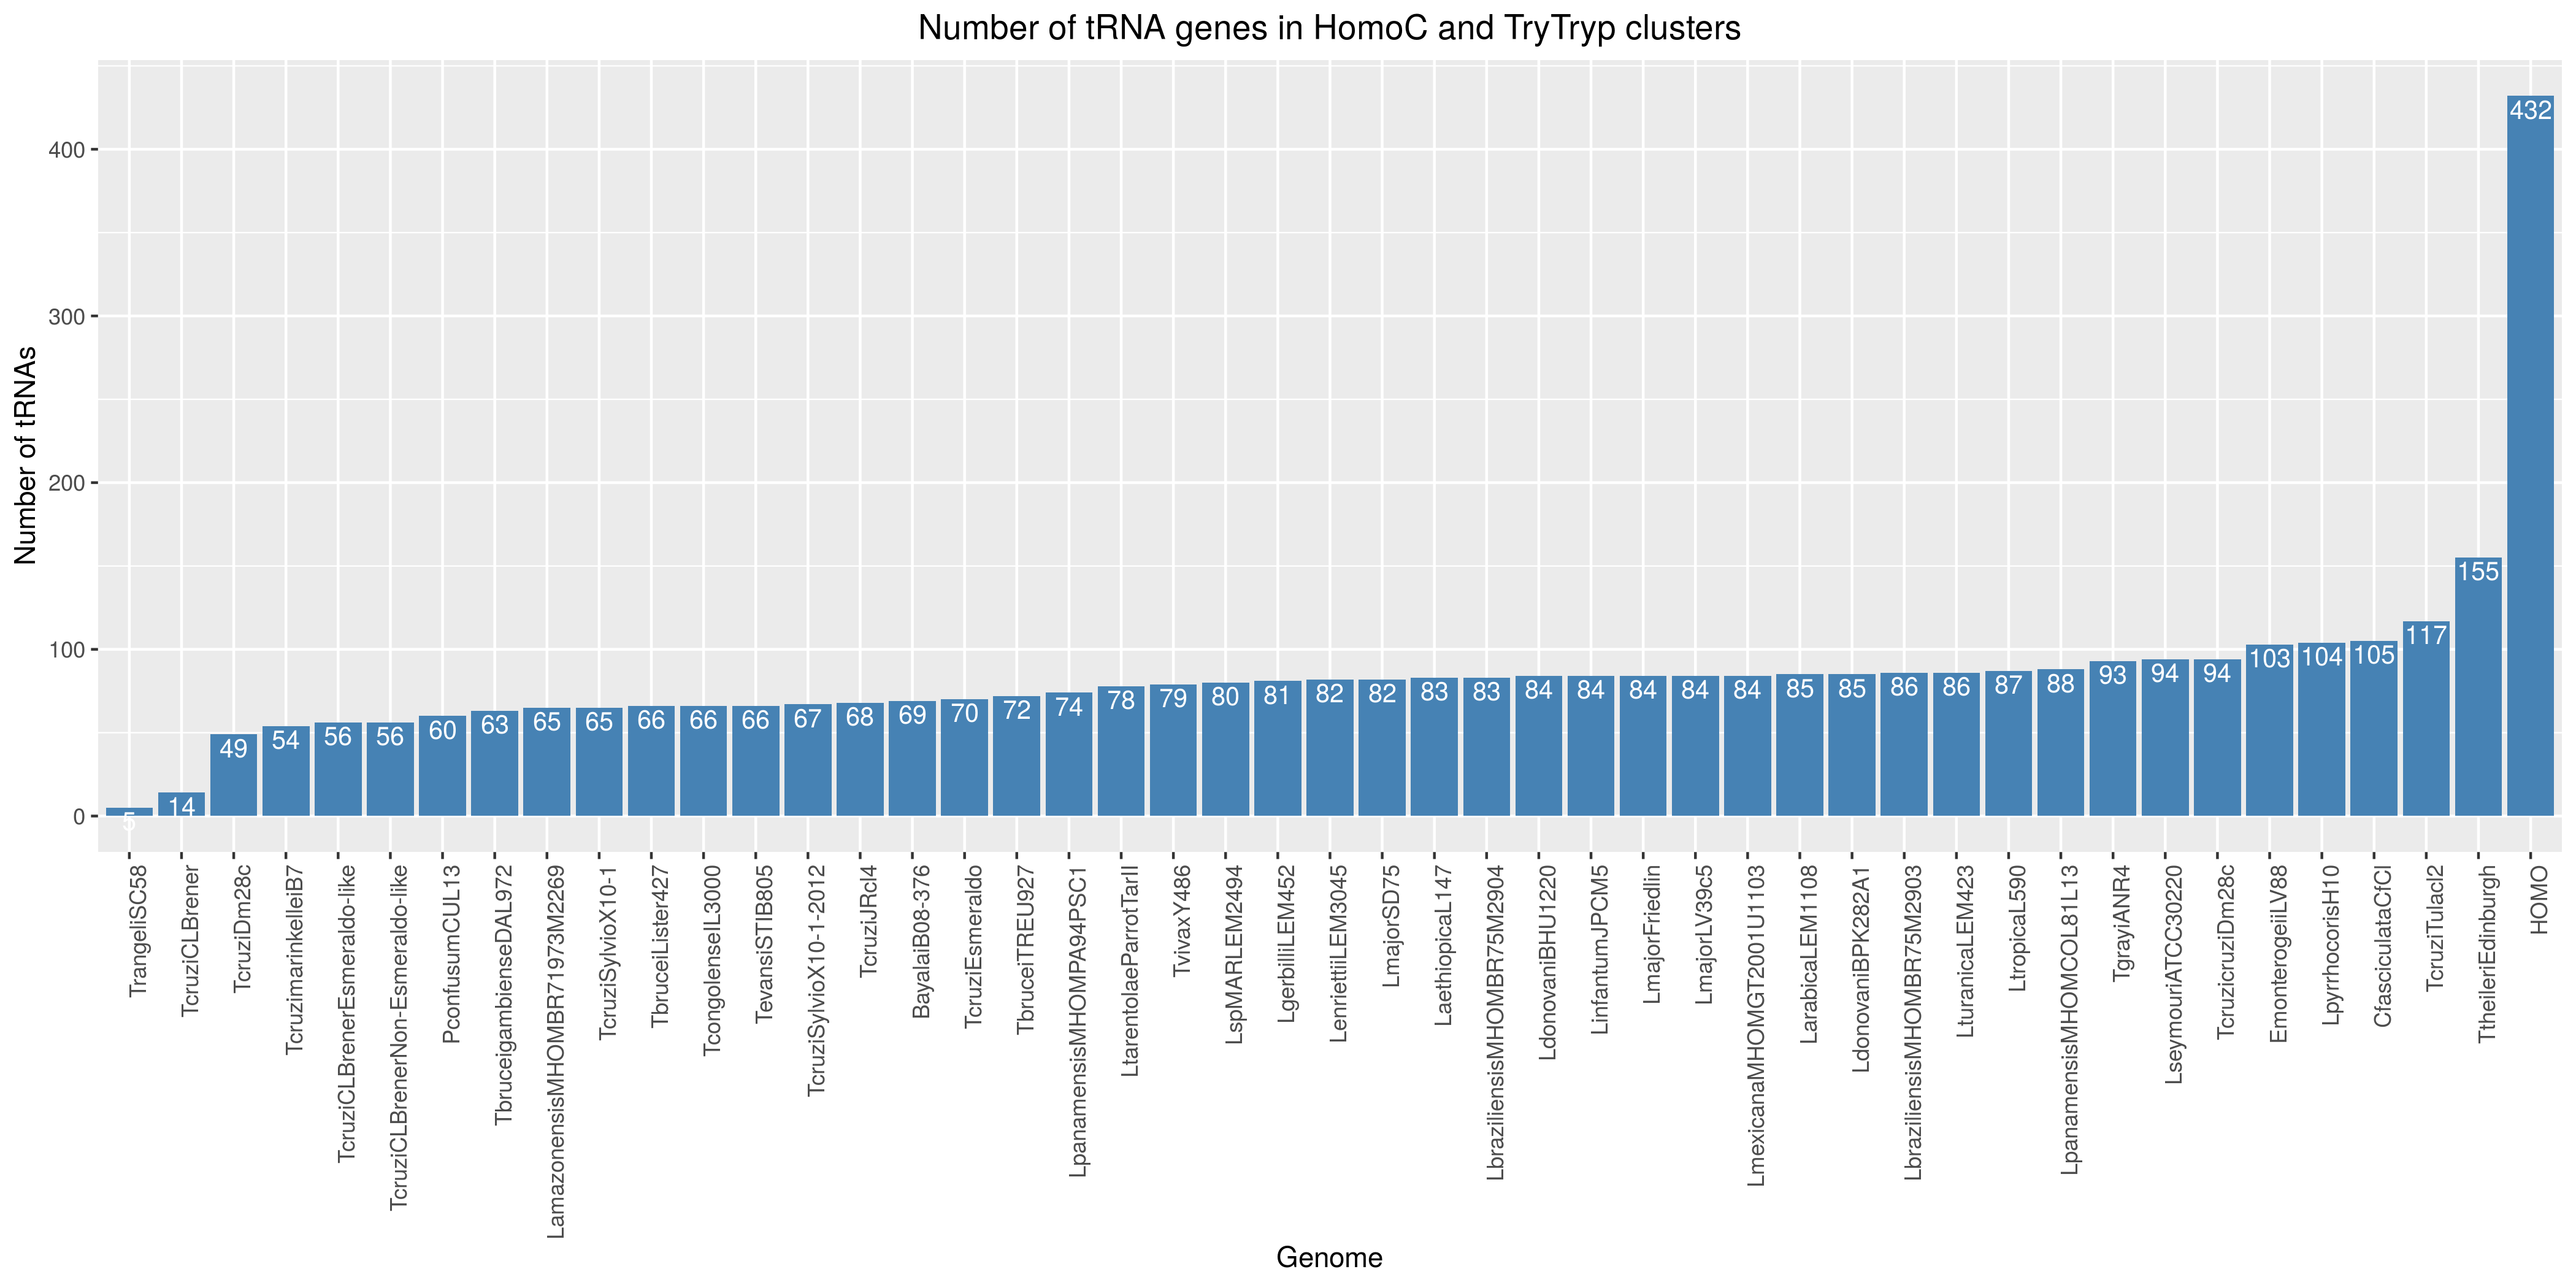
\includegraphics[width=0.8\columnwidth]{tRNAcounts_clustered.png} 
\caption[Number of Genes annotated]{Number of genes annotated by both TSE and ARA for each TryTryp cluster.}
\label{fig:countsclustered} 
\end{figure}

\begin{figure}[tb]
\centering 
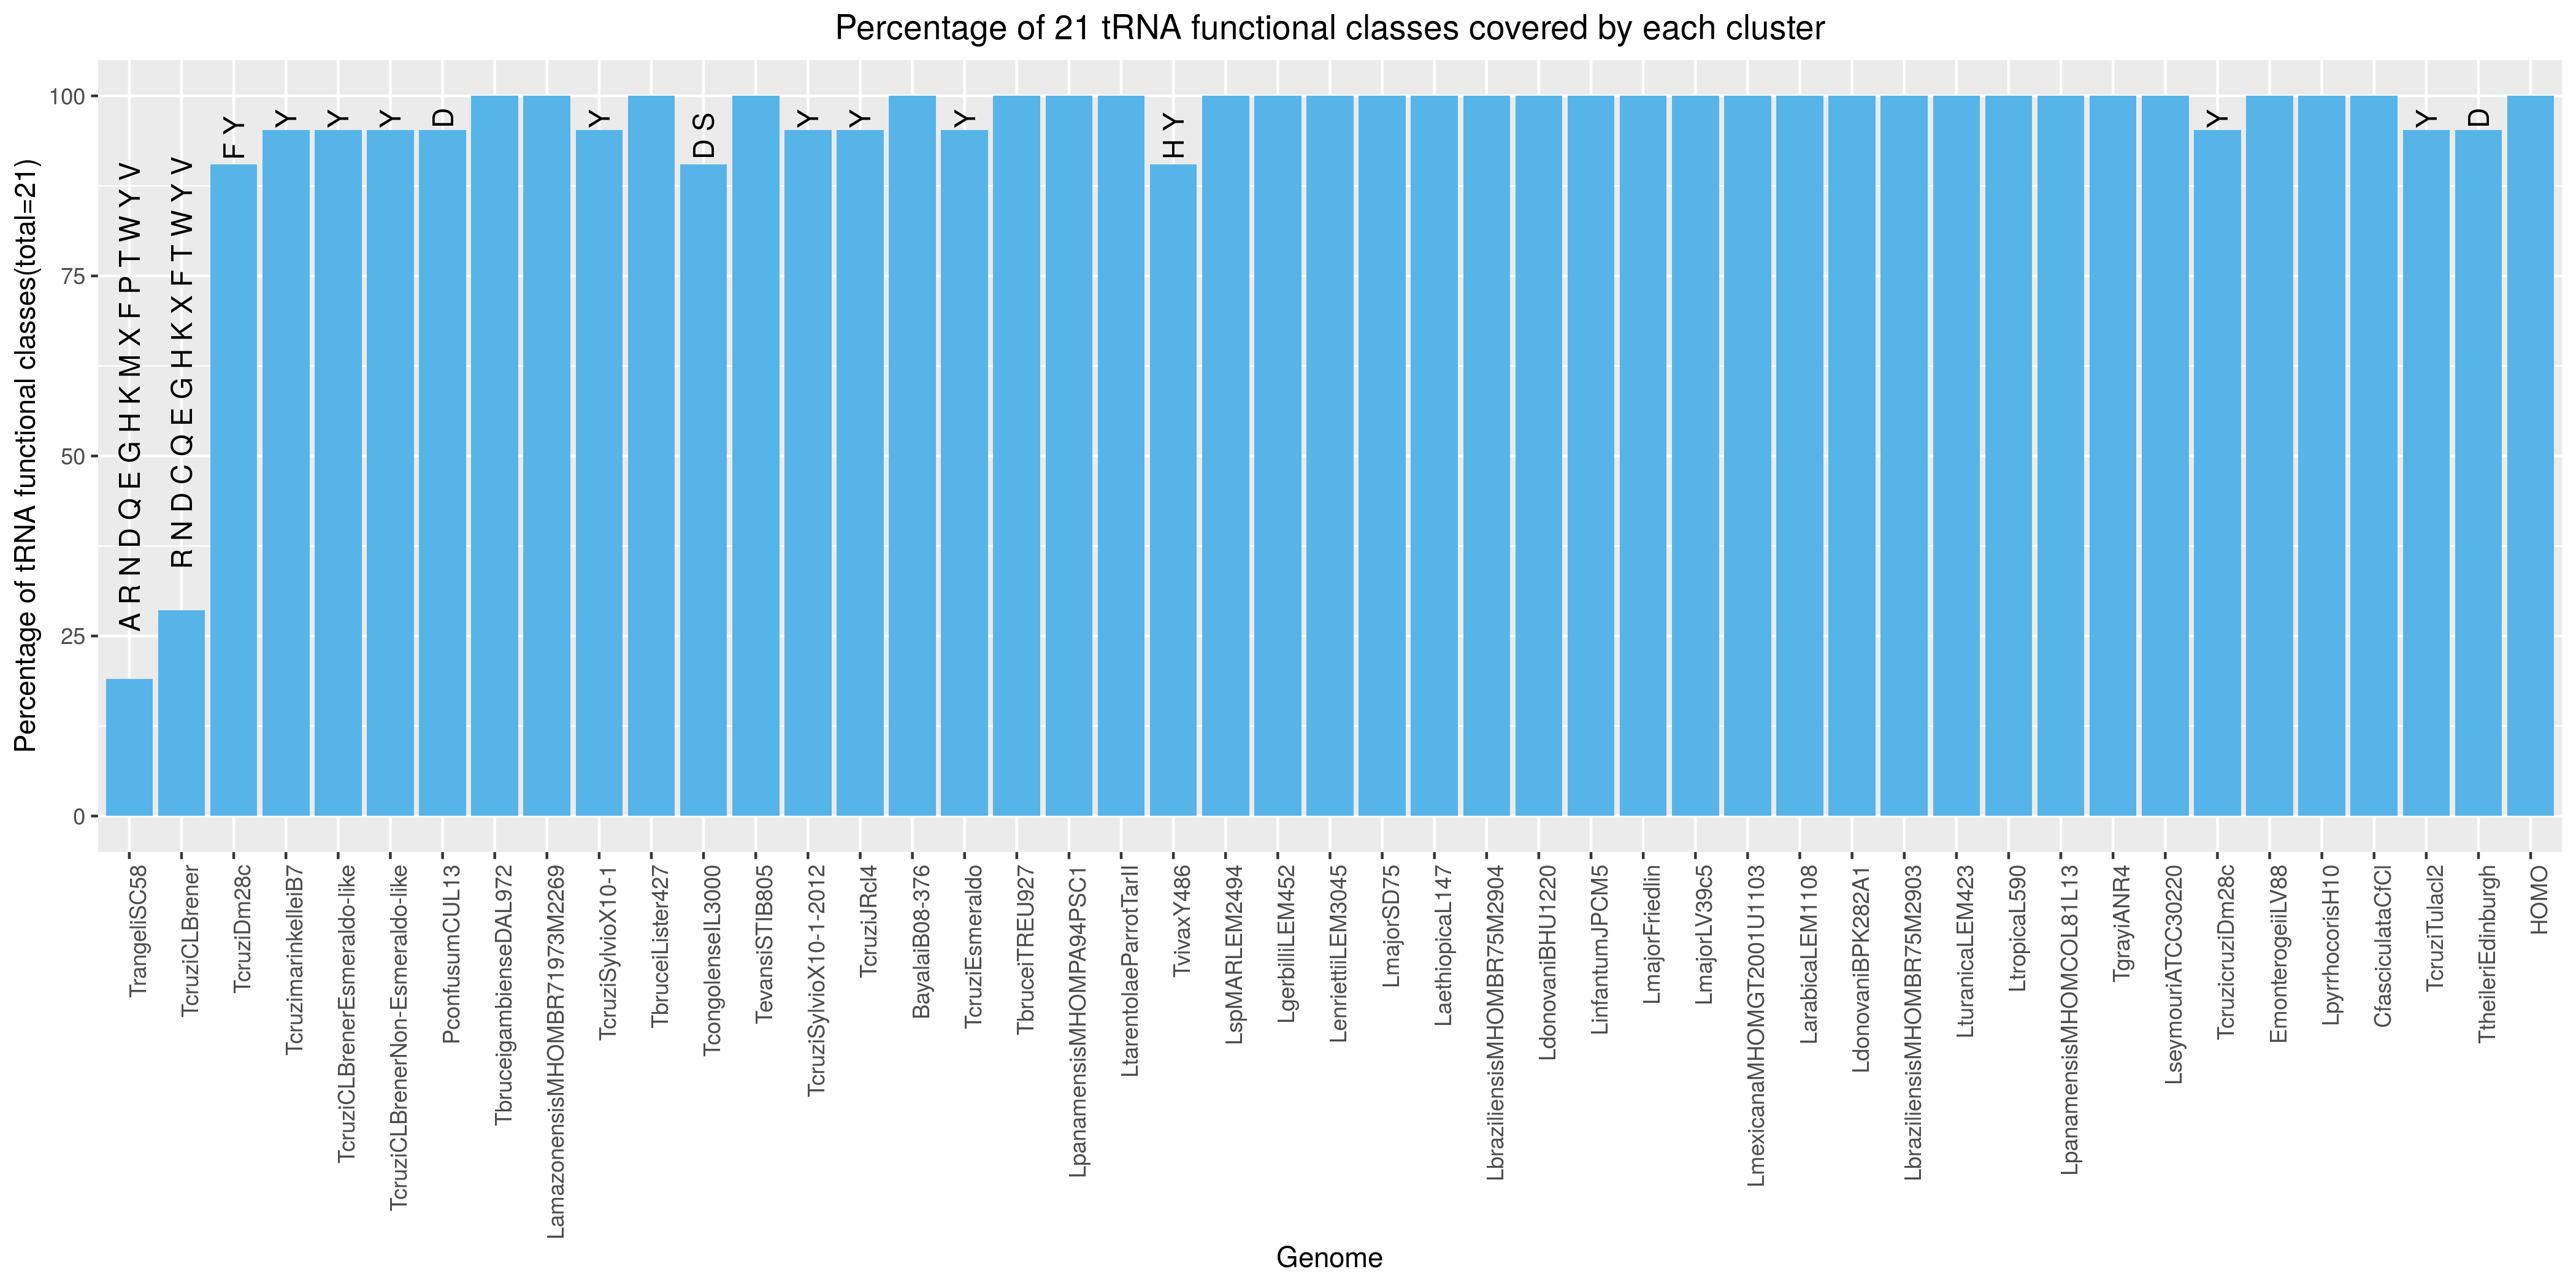
\includegraphics[width=0.8\columnwidth]{funcPerc_clustered.png} 
\caption[Genome Comparison]{Percentage of 22 tRNA types annotated by both TSE and ARA for each TryTryp cluster. The label on top of each bar shows which tRNA classes are not annotated for the genome.} 
\label{fig:funcclustered} 
\end{figure}
%----------------------------------------------------------------------------------------
%	BIBLIOGRAPHYyour own dat
%----------------------------------------------------------------------------------------
\newpage
\renewcommand{\refname}{\spacedlowsmallcaps{References}} % For modifying the bibliography heading

\bibliographystyle{unsrt}

\bibliography{sample.bib} % The file containing the bibliography

%----------------------------------------------------------------------------------------

\end{document}